%\documentclass{standalone}
%\usepackage{graphicx}
%\usepackage[usenames,dvipsnames,svgnames,table]{xcolor}
%\usepackage{tikz}
%\begin{document}
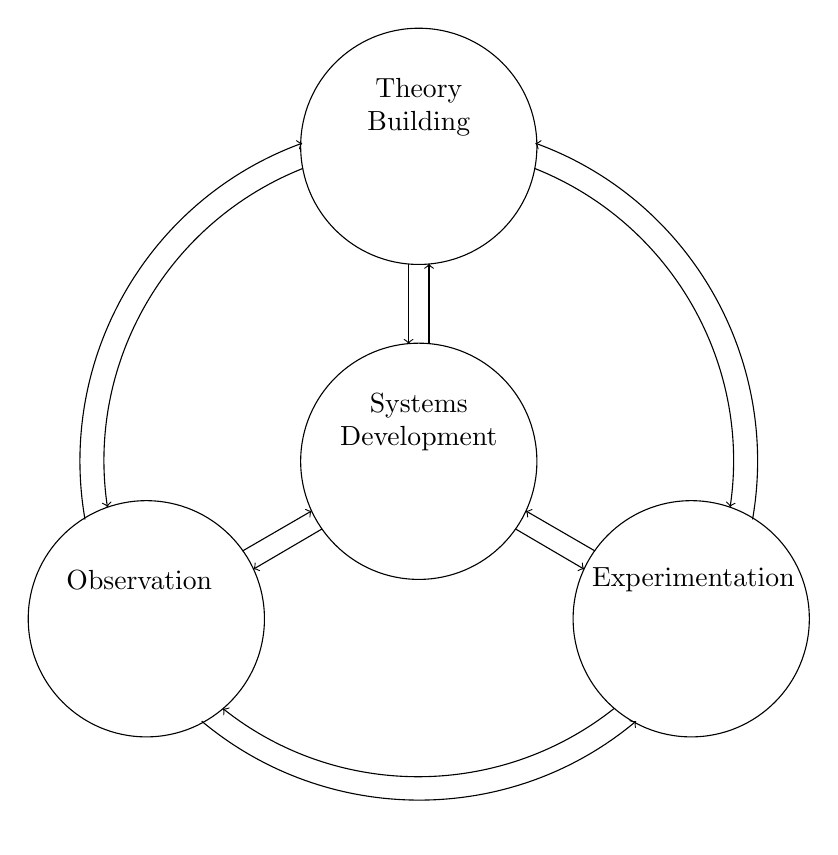
\begin{tikzpicture}[scale = 1]

% START: Rust generated
\draw [black] (0.00, 0.00) circle [radius=1.5];
\draw [black] (0.00, 4.00) circle [radius=1.5];
\draw [black] (3.46, -2.00) circle [radius=1.5];
\draw [black] (-3.46, -2.00) circle [radius=1.5];
\draw [->] (1.23, -0.86) -- (2.10, -1.37);
\draw [->] (2.24, -1.14) -- (1.36, -0.63);
\draw [->] (-1.23, -0.86) -- (-2.10, -1.37);
\draw [->] (-2.24, -1.14) -- (-1.36, -0.63);
\draw [->] (0.13, 1.49) -- (0.13, 2.51);
\draw [->] (-0.13, 2.51) -- (-0.13, 1.49);
\draw[->] (-1.47,3.72) arc [radius=4.00, start angle = 111.61, end angle = 188.39];
\draw[->] (1.47,3.72) arc [radius=4.00, start angle = 68.39, end angle = -8.39];
\draw[->] (2.48,-3.14) arc [radius=4.00, start angle = 308.39, end angle = 231.61];
\draw[<-] (-1.48,4.04) arc [radius=4.30, start angle = 110.09, end angle = 189.91];
\draw[<-] (1.48,4.04) arc [radius=4.30, start angle = 69.91, end angle = -9.91];
\draw[<-] (2.76,-3.30) arc [radius=4.30, start angle = 309.91, end angle = 230.09];

% END: Rust generated
\node[text width=2cm, align=center]  at (0,0.5) {Systems Development};
\node[text width=2cm, align=center]  at (0,4.5) {Theory Building};
\node[text width=2cm, align=center]  at (-3.55, -1.5) {Observation};
\node[text width=2cm, align=center]  at (3.2, -1.5) {Experimentation};

\end{tikzpicture}
%\end{document}
